% **************************************************************************************************
% **************************************************************************************************
\newsection{Floats: Graphics, Tables, and Listings}{intro:floats}



% **************************************************************************************************
\newsubsection{Figures and Tables}{intro:floats:figures}
Even relatively complex figures are easy to create, as you can see from this example. Note that you can refer to Figure~\ref{fig:intro:floats:usage:figure}, but also to the subfigures: Figure~\ref{fig:intro:floats:usage:figure-ex1} and Figure~\ref{fig:intro:floats:usage:figure-ex2}.
\begin{figure}
  \centering
  \subfigure[left side]{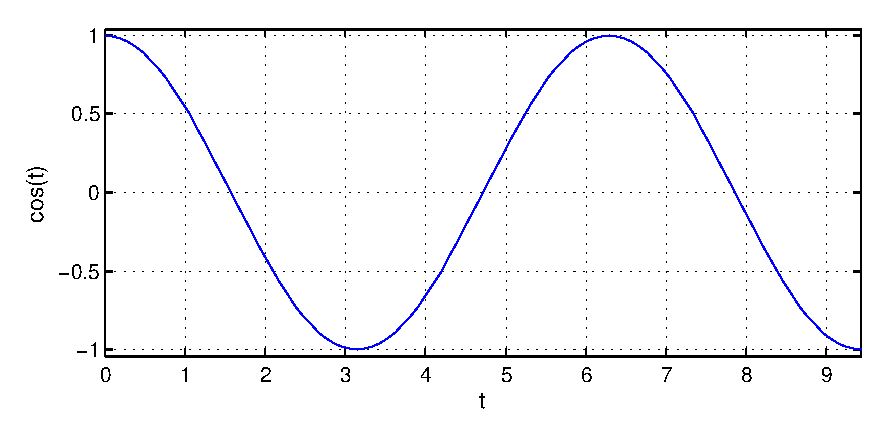
\includegraphics[width=0.495\textwidth]{\pwd/plots/example1}\label{fig:intro:floats:usage:figure-ex1}} \hfill
  \subfigure[right side]{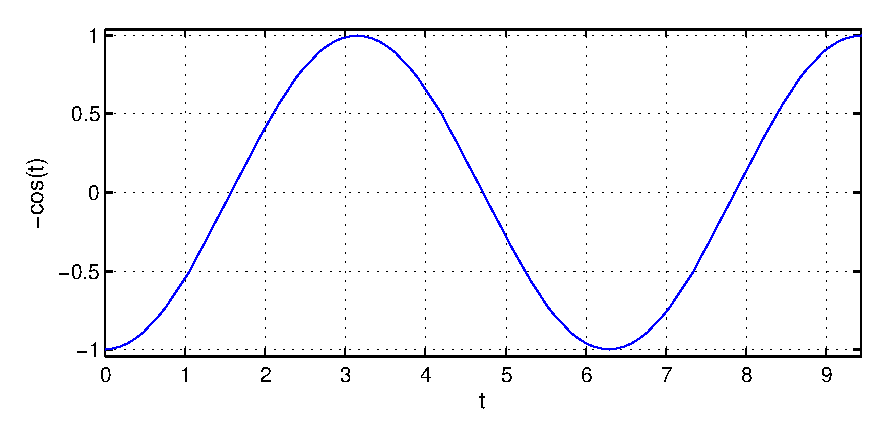
\includegraphics[width=0.495\textwidth]{\pwd/plots/example2}\label{fig:intro:floats:usage:figure-ex2}}
  \caption{Two subplots.}
  \label{fig:intro:floats:usage:figure}
\end{figure}

\noindent The same image can be created via a standardized command,
{\tiny\begin{verbatim}
  \twofigs{\pwd/plots/example1}{left side}{-ex1}{\pwd/plots/example2}{right side}{-ex2}{Two subplots.}{intro:floats:usage:figure-std}
\end{verbatim}}
\noindent and referenced like this: Fig.~\ref{fig:intro:floats:usage:figure-std}. There are several more standardized functions for figures, cf. Table~\ref{tab:intro:floats:figures}. Captions and labels are mandatory for all these commands.
\begin{longtable}{>{\tiny}l|>{\tiny}p{0.3\textwidth}}
  \normalsize\textbf{Command} & \normalsize\textbf{Description} \\\hline
  \verb|\fig{file}{caption}{label}| & Standard figure, full textwidth. \\\hline
  \verb|\figc{param}{file}{caption}{label}| & Standard figure with controllable parameters for includegraphics. \\\hline
  \verb|\twofig{file_l}{caption_l}{file_r}{caption_r}{caption}{label}| & Two figures, side by side. \\\hline
  \verb|\twofigs{file_l}{caption_l}{add.label_l}{filename_r}{caption_r}{add.label_l}{caption}{label}| & Two figures, side by side, with labels for each subfigure. Figure~\ref{fig:intro:floats:usage:figure-std} is created by this command.\\\hline
  \verb|\twofigc{param_l}{file_l}{caption_l}{param_l}{filename_r}{caption_r}{caption}{label}| & Two figures, side by side, with controllable parameters for includegraphics. \\\hline
  \verb|\figf|, \verb|\figcf|, \verb|\twofigf|, \verb|\twofigsf|, \verb|\twofigcf| & Like the above, but with framed figures. \\
  \caption{Standardized commands for figures.}
  \label{tab:intro:floats:figures}
\end{longtable}

\twofigs{\pwd/plots/example1}{left side}{-ex1}{\pwd/plots/example2}{right side}{-ex2}{Two subplots.}{intro:floats:usage:figure-std}



% **************************************************************************************************
\newsubsection{Listings}{intro:floats:listings}

\filelisting{matlab}{\pwd/plots/matlab.m}{Some matlab code example (highlighting can be configured).}{code-example}